
%(BEGIN_QUESTION)
% Copyright 2012, Tony R. Kuphaldt, released under the Creative Commons Attribution License (v 1.0)
% This means you may do almost anything with this work of mine, so long as you give me proper credit

Interpret the pressure measurement displayed by this gauge mechanism, assuming a gauge accuracy of $\pm$ 2\% full scale:

$$\epsfxsize=6in 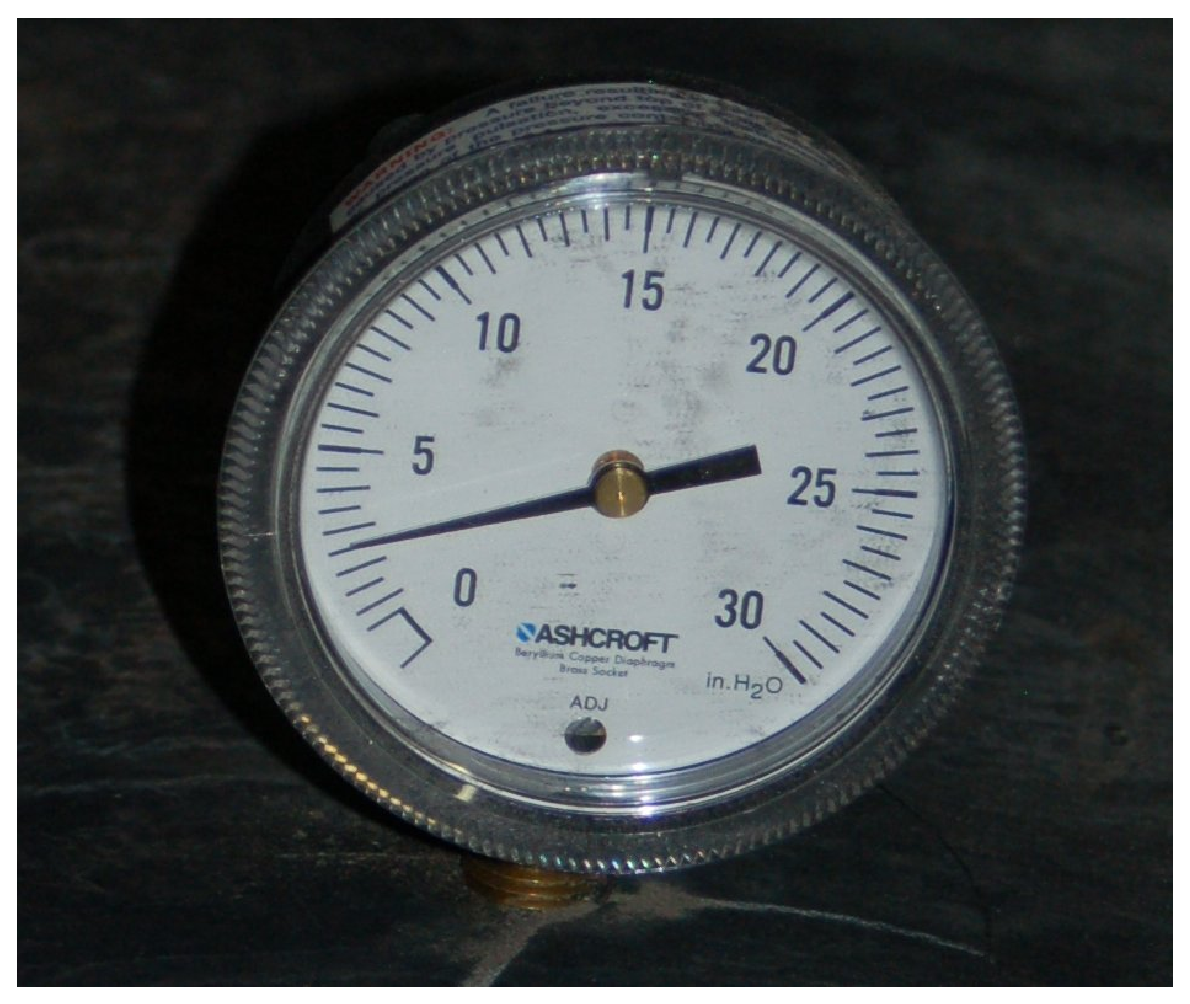
\includegraphics[width=15.5cm]{i01155x01.eps}$$

How low and how high could this pressure actually be, given the stated accuracy of this gauge?

\underbar{file i01155}
%(END_QUESTION)





%(BEGIN_ANSWER)

Pressure = 2.5 "H$_{2}$O $\pm$ 0.6 "H$_{2}$O.  This means the actual pressure could be as low as 1.9 "H$_{2}$O or as high as 3.1 "H$_{2}$O.

 
\vskip 10pt

If you look closely at the photograph, you can see that the camera's angle to the gauge face is not straight-on, and therefore there will be some {\it parallax error} in reading this gauge's face.  If we were to lower the camera's view to get a more direct look at the gauge, we might see the needle pointing between the 2.5 and 3 divisions, which would mean a pressure of 2.75 "H$_{2}$O $\pm$0.6 "H$_{2}$O.

%(END_ANSWER)





%(BEGIN_NOTES)


%INDEX% Measurement, analog gauge reading

%(END_NOTES)


